% Method overview compiled directly by the manuscript.
% The vertical organization mirrors the logic of the construction rather than
% compressing all ingredients into one horizontal strip.
% Model colours match the data figures: ICNN green, ICKAN blue.  Components
% shared by both cores stay neutral.
\definecolor{icnncolor}{HTML}{2AA780}%
\definecolor{ickancolor}{HTML}{2B5DAA}%
\begin{tikzpicture}[x=1cm,y=1cm,font=\small,
  panel/.style={draw=black!55,rounded corners=2pt,line width=.55pt,fill=white},
  flow/.style={-{Latex[length=2mm]},draw=black!70,line width=.8pt},
  secondaryflow/.style={-{Latex[length=1.8mm]},draw=black!55,line width=.7pt},
  stage/.style={circle,draw=black!60,fill=black!72,text=white,
                font=\bfseries\footnotesize,minimum size=5.2mm,inner sep=0pt},
  dot/.style={circle,fill=black,inner sep=0pt,minimum size=3.8pt},
  sum/.style={circle,draw=black!65,fill=black!6,
              minimum size=3.7mm,inner sep=0pt},
  weight/.style={draw=icnncolor!90!black,line width=.75pt},
  connection/.style={draw=black!55,line width=.5pt},
  inputmap/.style={draw=violet!65!black,dashed,line width=.55pt},
  pics/softplus/.style={code={
    \draw[draw=black!55,fill=white,line width=.45pt]
      (-.38,-.27) rectangle (.38,.27);
    \draw[black!22,line width=.2pt]
      (-.29,-.18)--(.29,-.18) (-.29,-.18)--(-.29,.19);
    \draw[black!70,line width=.62pt]
      plot[domain=-3:3,samples=30]
      ({.095*\x},{-.18+.34*(ln(1+exp(\x))-ln(1+exp(-3)))/3});
  }},
  pics/edgecurve/.style args={#1}{code={
    \draw[draw=ickancolor,fill=white,line width=.42pt]
      (-.38,-.27) rectangle (.38,.27);
    \draw[black!22,line width=.2pt]
      (-.29,-.18)--(.29,-.18) (-.29,-.18)--(-.29,.19);
    \draw[ickancolor!85!black,line width=.62pt]
      plot[domain=-1.5:1.5,samples=30]
      ({.19*\x},{-.18+.03*(\x+1.5)+#1*.045*(\x+1.5)*(\x+1.5)});
  }}
]
 \path[use as bounding box] (0,0) rectangle (16.2,15.65);

 % The first two levels are drawn in their original frame and shifted down
 % to sit directly above the analytic completion.
 \begin{scope}[yshift=-4.89cm]
 % -------------------------------------------------------------------------
 % First level: an actual RVE response and the directional description.
 \node[panel,minimum width=6.00cm,minimum height=5.00cm,anchor=south west]
   (rvepanel) at (0,15.50) {};
 \node[stage] at (.36,20.12) {1};
 \node[font=\small\bfseries,anchor=west] at (.74,20.12)
   {Sampling and RVE data};
 \node[inner sep=0pt] at (1.32,17.92)
   {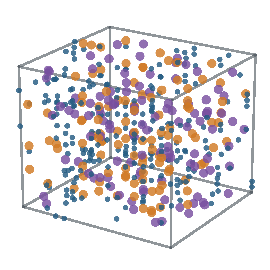
\includegraphics[width=2.45cm]{sampling_material_a_overview.pdf}};
 \node[font=\scriptsize,text=black!65] at (1.32,15.98)
   {strain samples $\{\ee^s\}$};
 \draw[flow] (2.56,17.95)--(3.02,17.95);
 \node[font=\tiny,text=black!60] at (2.79,18.20) {FOM};
 \node[inner sep=0pt] at (4.52,17.95)
   {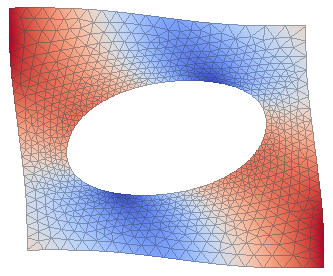
\includegraphics[width=3.05cm]{rve_deformed_overview.pdf}};
 \node[font=\scriptsize] at (4.52,15.98)
   {$\F^{s}\mapsto\bigl(W^{s},\ssv^{s}\bigr)$};

 \node[panel,minimum width=9.65cm,minimum height=5.00cm,anchor=south west,
       fill=orange!1] (featurepanel) at (6.45,15.50) {};
 \node[stage] at (6.81,20.12) {2};
 \node[font=\small\bfseries,anchor=west] at (7.19,20.12)
   {Learnable paired directional features};

 % Each sensor is explicitly drawn on the undeformed discretized RVE.
 \foreach \yy/\lab/\ang in {19.18/{z_1}/24,17.84/{z_2}/-12,16.25/{z_m}/48} {
   \node[inner sep=0pt] at (7.72,\yy)
     {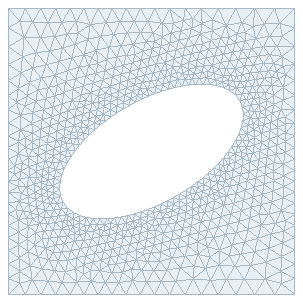
\includegraphics[width=.96cm]{rve_reference_overview.pdf}};
   \node[font=\scriptsize,anchor=east] at (7.17,\yy) {$\lab$};
   \coordinate (sensor) at (7.72,\yy);
   \draw[orange!85!black,line width=.85pt,-{Latex[length=1.1mm]}]
     (sensor)--++(\ang:.31);
   \draw[teal!75!black,line width=.85pt,-{Latex[length=1.1mm]}]
     (sensor)--++({\ang+90}:.31);
   \fill (sensor) circle (.85pt);
 }
 \node[font=\normalsize] at (7.72,17.04) {$\vdots$};

 \node[align=center,font=\small] at (11.90,17.68)
   {$\displaystyle z_i(\F,J)
     =\frac{\|\F\bm d_i\|^{2p_i}}{p_iJ^{b_i}}
     +\frac{\|\F\bm d_i^\perp\|^{2q_i}}{q_iJ^{c_i}}$};
 \node[align=center,font=\scriptsize,text=black!62] at (11.90,16.55)
   {orientation and exponents adapt to the RVE response\\
    within the analytic convexity bounds};
 \draw[orange!85!black,line width=.9pt,-{Latex[length=1.2mm]}]
   (11.30,19.12)--++(.55,0);
 \node[font=\scriptsize,anchor=west] at (11.99,19.12) {$\bm d_i$};
 \draw[teal!75!black,line width=.9pt,-{Latex[length=1.2mm]}]
   (11.30,18.62)--++(.55,0);
 \node[font=\scriptsize,anchor=west] at (11.99,18.62) {$\bm d_i^\perp$};

 \draw[flow] (rvepanel.east)--(featurepanel.west);

 \begin{scope}[yshift=.05cm]
 % -------------------------------------------------------------------------
 % Second level: a small, horizontal version of the core-architecture figure.
 % Information flows from left to right; ellipses stand for intervening layers.
 \node[panel,minimum width=16.10cm,minimum height=3.60cm,anchor=south west]
   (corepanel) at (0,11.40) {};
 \node[stage] at (.36,14.62) {3};
 \node[font=\small\bfseries,anchor=west] at (.74,14.62)
   {Monotone convex core};
 \draw[black!18] (8.05,11.60)--(8.05,14.35);
 \draw[flow] (featurepanel.south) -- (11.28,15.00);
 \node[font=\scriptsize,text=black!65,anchor=west] at (11.42,15.225)
   {conditioned input $\bm y(\bm z)$};

 % ICNN: learned nonnegative weights feed fixed softplus nodes.
 \node[font=\scriptsize\bfseries,text=icnncolor!80!black] at (4.03,14.10) {ICNN};
 \node[font=\scriptsize,text=black!65] at (4.03,13.76)
   {learned nonnegative weights, fixed softplus on nodes};
 \foreach \lx in {2.88,4.58}
   \filldraw[black!45,fill=black!3,line width=.6pt,rounded corners=1pt]
     (\lx-.33,11.92) rectangle (\lx+.33,13.40);
 \node[dot] (icin1) at (1.68,13.14) {};
 \node[dot] (icinm) at (1.68,12.18) {};
 \node[font=\scriptsize,anchor=east] at (1.56,13.14) {$y_1$};
 \node[font=\scriptsize,anchor=east] at (1.56,12.18) {$y_m$};
 \node[font=\scriptsize] at (1.68,12.72) {$\vdots$};
 \node[dot] (icout) at (5.78,12.66) {};
 \foreach \ya in {13.14,12.66,12.18} {
   \draw[weight] (icin1)--(2.644,\ya);
   \draw[weight] (icinm)--(2.644,\ya);
   \draw[weight] (4.816,\ya)--(icout);
   \foreach \yb in {13.14,12.66,12.18}
     \draw[weight] (3.116,\ya)--(4.344,\yb);
 }
 \fill[white] (3.53,11.95) rectangle (3.93,13.37);
 \foreach \ya in {13.14,12.66,12.18}
   \node[font=\scriptsize] at (3.73,\ya) {$\cdots$};
 \foreach \lx in {2.88,4.58}
   \foreach \ya in {13.14,12.66,12.18}
     \pic[scale=.62] at (\lx,\ya) {softplus};
 \node[font=\scriptsize,anchor=west] at (5.90,12.66) {$\widehat H(\bm y)$};
 % The conditioned input also enters the last hidden layer and the output.
 \draw[inputmap,rounded corners=2pt,-{Latex[length=1.1mm]}]
   (icinm)--(1.68,11.62)--(5.78,11.62)--(icout);
 \draw[inputmap,-{Latex[length=1mm]}] (4.58,11.62)--(4.58,11.90);

 % ICKAN: every edge carries its own learned convex, nondecreasing function.
 \node[font=\scriptsize\bfseries,text=ickancolor] at (12.08,14.10) {ICKAN};
 \node[font=\scriptsize,text=black!65] at (12.08,13.76)
   {learned convex, nondecreasing functions on edges};
 \filldraw[ickancolor,fill=ickancolor!4,line width=.6pt,rounded corners=1pt]
   (10.28,11.80) rectangle (10.72,13.52);
 \filldraw[ickancolor,fill=ickancolor!4,line width=.6pt,rounded corners=1pt]
   (12.76,11.98) rectangle (13.24,13.34);
 \node[dot] (kin1) at (9.80,13.14) {};
 \node[dot] (kinm) at (9.80,12.18) {};
 \node[font=\scriptsize,anchor=east] at (9.68,13.14) {$y_1$};
 \node[font=\scriptsize,anchor=east] at (9.68,12.18) {$y_m$};
 \node[font=\scriptsize] at (9.80,12.72) {$\vdots$};
 \foreach \j/\yn in {1/13.14,2/12.66,3/12.18} {
   \node[dot] (kfirst\j) at (11.30,\yn) {};
   \node[dot] (klast\j) at (12.35,\yn) {};
 }
 \node[dot] (kout) at (13.70,12.66) {};
 \foreach \j/\ya/\yb in {1/13.36/13.08,2/12.80/12.52,3/12.24/11.96} {
   \draw[connection] (kin1)--(10.50,\ya)--(kfirst\j);
   \draw[connection] (kinm)--(10.50,\yb)--(kfirst\j);
 }
 \foreach \j/\yn in {1/13.14,2/12.66,3/12.18} {
   \foreach \k in {1,2,3}
     \draw[connection] (kfirst\j)--(klast\k);
   \draw[connection] (klast\j)--(13.00,\yn)--(kout);
 }
 \fill[white] (11.63,11.95) rectangle (12.03,13.37);
 \foreach \yn in {13.14,12.66,12.18}
   \node[font=\scriptsize] at (11.83,\yn) {$\cdots$};
 \foreach \yy/\cc in {13.36/.70,13.08/.55,12.80/.80,12.52/.60,12.24/.75,11.96/.50}
   \pic[scale=.40] at (10.50,\yy) {edgecurve=\cc};
 \foreach \yy/\cc in {13.14/.72,12.66/.58,12.18/.66}
   \pic[scale=.45] at (13.00,\yy) {edgecurve=\cc};
 \node[font=\scriptsize,anchor=west] at (13.82,12.66) {$\widehat H(\bm y)$};
 % As in the deployed ICKAN, the conditioned input also has an output map.
 \draw[inputmap,rounded corners=2pt,-{Latex[length=1.1mm]}]
   (kinm)--(9.80,11.62)--(13.70,11.62)--(kout);
 \end{scope}
 \end{scope}

 % Both alternatives produce the same learned scalar contribution.
 \node[panel,minimum width=3.70cm,minimum height=.82cm]
   (hcore) at (8.05,5.89) {};
 \node[font=\scriptsize,align=center] at (8.05,5.98)
   {$H(\bm z)=\widehat H\!\left(\bm y(\bm z)\right)$};
 \node[font=\scriptsize,text=black!60] at (8.05,5.71)
   {learned contribution};
 \draw[secondaryflow] (corepanel.south)--(hcore.north);

 % -------------------------------------------------------------------------
 % Third level: analytic completion is part of the complete energy itself.
 \node[panel,minimum width=11.05cm,minimum height=3.60cm,
       anchor=south west] (energy) at (0,1.28) {};
 \node[stage] at (.36,4.49) {4};
 \node[font=\small\bfseries,anchor=west] at (1.08,4.49)
   {Complete stored energy};

 \node[font=\small,align=left] at (5.53,2.98)
   {$\displaystyle W(\F)=
      \underbrace{H(\bm z)-H(\bm z^0)}_{W_{\rm learn}}
      \underbrace{-r(J-1)}_{W_{\rm corr}}$\\[5pt]
    $\displaystyle \qquad+
      \underbrace{\alpha(J-1-\log J)+\frac{\beta}{2}(J-1)^2}_{W_{\rm vol}}
      +\underbrace{\varepsilon\!\left(\frac{\operatorname{tr}\C}{2}-1-\log J\right)}_{W_{\rm dist}}$};
 \node[font=\scriptsize,text=black!60] at (5.53,1.56)
   {reference state: $W(\I)=0,\qquad \ssv(\bm0)=\bm0$};

 \node[panel,minimum width=4.60cm,minimum height=3.60cm,
       anchor=south west] (response) at (11.50,1.28) {};
 \node[stage] at (11.87,4.49) {5};
 \node[font=\small\bfseries,anchor=west] at (12.25,4.49)
   {Constitutive output};
 \node[font=\small] at (13.80,3.38)
   {$\underbrace{\ssv=\nabla_{\ee}W}_{\text{stress}}$};
 \node[font=\small] at (13.80,2.05)
   {$\underbrace{\bm D=\nabla_{\ee}^{2}W}_{\text{tangent}}$};

 \draw[secondaryflow,rounded corners=2pt]
   (hcore.south) -- ++(0,-.22) -| (energy.north);
 \draw[flow] (energy.east)--(response.west);

 % Guarantee ribbon.  The six equally spaced entries reproduce criteria
 % (C1)--(C6) exactly; their labels replace manually positioned separators.
 \node[panel,fill=black!3,minimum width=16.10cm,minimum height=1.12cm]
   at (8.05,.60) {};
 \node[font=\footnotesize\bfseries] at (8.05,.96)
   {Criteria satisfied by construction};
 \node[font=\scriptsize,align=center,text=black!75]
   at (1.43,.43) {\textbf{(C1)} potential\\structure};
 \node[font=\scriptsize,align=center,text=black!75]
   at (4.08,.43) {\textbf{(C2)}\\objectivity};
 \node[font=\scriptsize,align=center,text=black!75]
   at (6.73,.43) {\textbf{(C3)} stress symmetry\\and anisotropy};
 \node[font=\scriptsize,align=center,text=black!75]
   at (9.38,.43) {\textbf{(C4)} reference\\normalization};
 \node[font=\scriptsize,align=center,text=black!75]
   at (12.03,.43) {\textbf{(C5)} 2D\\polyconvexity};
 \node[font=\scriptsize,align=center,text=black!75]
   at (14.68,.43) {\textbf{(C6)}\\growth};
\end{tikzpicture}
